%\documentclass[a4paper, 10pt,twocolumn]{article}
\documentclass[a4paper, 10pt]{article}
\usepackage[margin=1in]{geometry}
\usepackage{graphicx}
\usepackage{float}
\usepackage{mathtools}
\usepackage{amsmath}
\usepackage{subfigure}
\usepackage{color}
\usepackage[usenames,dvipsnames,svgnames,table]{xcolor}
\usepackage{amssymb}
\usepackage{pifont}
\usepackage[english]{babel}
\usepackage[hidelinks]{hyperref}
\usepackage{fancyvrb}
\usepackage{bera}
\newcommand{\cmark}{\ding{51}}%
\newcommand{\xmark}{\ding{55}}%

\usepackage[utf8]{inputenc}
\usepackage[english]{babel}
 
\setlength{\parindent}{0em}
\setlength{\parskip}{0em}

\usepackage{listings}
\usepackage{color} %red, green, blue, yellow, cyan, magenta, black, white
\definecolor{mygreen}{RGB}{28,172,0} % color values Red, Green, Blue
\definecolor{mylilas}{RGB}{170,55,241}
% Using typewriter font: \ttfamily inside \lstset
\lstset{language=Matlab,%
    %basicstyle=\color{red},
    breaklines=true,%
    morekeywords={matlab2tikz},
    keywordstyle=\color{blue},%
    morekeywords=[2]{1}, keywordstyle=[2]{\color{black}},
    identifierstyle=\color{black},%
    stringstyle=\color{mylilas},
    commentstyle=\color{mygreen},%
    showstringspaces=false,%without this there will be a symbol in the places where there is a space
    basicstyle=\small\ttfamily,
    %numbers=left,%
    numberstyle={\tiny \color{black}},% size of the numbers
    numbersep=9pt, % this defines how far the numbers are from the text
    tabsize=4,
    emph=[1]{for,end,break},emphstyle=[1]\color{red}, %some words to emphasise
    %emph=[2]{word1,word2}, emphstyle=[2]{style},    
}

\begin{document}
\title{Visual Perception Lab report \\ \#2 Camera Calibration}
\author{Kaisar Kushibar\\
Master of Computer VIsion and RoBOTics (ViBot)\\University of Girona (Girona)}

\maketitle
%------------------------------------
\section*{Introduction}
In this laboratory work we are going review camera calibration methods and use Hall and Fougeras-Toscani methods to calibrate a simulated camera. We will also study the accuracy of these methods for different amount of additive noise in points on an image. The coursework consist of three parts and each part contains several steps. At each step we will give detailed explanation of our solution and also provide MATLAB code.
\section{Part 1}
This part consist of calibrating a simulated camera with parameters defined in Step\#1 (\ref{step1}).
\subsection{Step 1}\label{step1}
We are given the following camera parameters: (1) au, av ($\alpha_u, \alpha_v$) defined as $\alpha_u=-fk_u$ and $\alpha_v=-fk_v$, where $f$ is focal distance of the camera lens and $k_u$ and $k_v$ are parameters that convert metric distance to pixel; (2) u0, v0 ($u_0, v_0$) - components that translate coordinate center from camera focal point to image plane defined in top-left corner; (3) $T_x, T_y, T_z$ - translation of camera center from the world coordinate system; (4) Phix, Phiy, Phix1 ($\varphi_x, \varphi_y, \varphi_{x1}$) - rotation of the camera coordinate system with respect to world coordinate system and the rotation transformation is done in Euler $XYX$. We are also given the image size in pixels and we will use it in Step\#12 (\ref{step12})
\subsection{Step 2}\label{step2}
In this section we will define the intrinsic and extrinsic transformation matrices of the simulated camera given with parameters that were defined in the previous step. Before providing the MATLAB code let us tell a word about the use of these matrices. Intrinsic transformation matrix is used to change the coordinates from camera to computer image whereas extrinsic transformation matrix is used to change from world coordinate system to camera. Combining these two matrices we get a complete model of the camera. The listing below defines these two transformation matrices. \textbf{WRITE ABOUT THE ROTATION MATRICES, WHY ARE YOU CALCULATING THEM?}
\begin{lstlisting}
%intrinsic transformation matrix
intMat = [au 0 u0 0; 0 av v0 0; 0  0  1 0];
%extrinsic transformation matrix; Use Euler XYX1
rx = [1 0 0; 0 cos(Phix) -sin(Phix); 0 sin(Phix) cos(Phix)];
ry = [cos(Phiy) 0 sin(Phiy); 0 1 0; -sin(Phiy) 0 cos(Phiy)];
rx1 = [1 0 0; 0 cos(Phix1) -sin(Phix1); 0 sin(Phix1) cos(Phix1)];
R = rx*ry*rx1;
extMat = [R(1,:), tx; R(2,:), ty; R(3,:), tz; 0 0 0 1];
\end{lstlisting}
%\begin{lstlisting}
%%intrinsic transformation matrix
%intMat = [au 0 u0 0;
%          0 av v0 0;
%          0  0  1 0];
%%extrinsic transformation matrix; Use Euler XYX1
%rx = [1 0 0;
%      0 cos(Phix) -sin(Phix);
%      0 sin(Phix) cos(Phix)];
%
%ry = [cos(Phiy) 0 sin(Phiy);
%      0 1 0;
%      -sin(Phiy) 0 cos(Phiy)];
%rx1 = [1 0 0;
%       0 cos(Phix1) -sin(Phix1);
%       0 sin(Phix1) cos(Phix1)];
%R = rx*ry*rx1;
%extMat = [R(1,:), tx;
%          R(2,:), ty;
%          R(3,:), tz;
%          0 0 0 1];
%\end{lstlisting}
\subsection{Step 3}\label{step3}
In this step we define $pN$ random points in 3D in range [-480, 480] and create homogeneous coordinates from those points.
\begin{lstlisting}
pN = 6 % number of 3D points.
points3d = [randi([-480, 480], [pN, 1]), randi([-480, 480], [pN, 1]), randi([-480, 480], [pN, 1])];
% make homogeneous points from 3d points
hgPoints = points3d';
hgPoints(4,:) = 1;
\end{lstlisting}
\subsection{Step 4}\label{step4}
The script below computes projection of generated 3D points on the image plane. We use homogeneous coordinates for the computation and normalize the projections.
\begin{lstlisting}
proj = intMat*extMat*hgPoints;
projNorm = zeros(2, pN);
projNorm(1,:) = proj(1,:)./proj(3,:);
projNorm(2,:) = proj(2,:)./proj(3,:);
\end{lstlisting}
\subsection{Step 5}\label{step5}
The figure below illustrates the projected points on the image plane.
\begin{figure}[H]
\centering
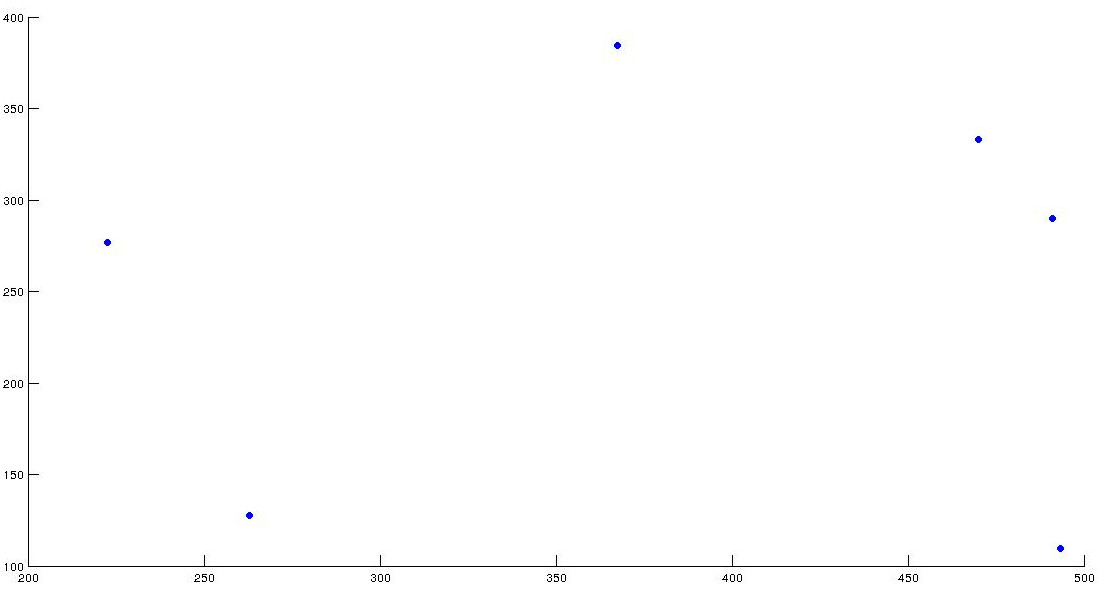
\includegraphics[width=4in]{./pics/step5}
\caption{Projection of 3D points on the image plane.}
\label{fig:step5}
\end{figure}
As it can be seen from the figure above, the points are not distributed well on the image plane, because of the less number of points. The distribution of points might affect the accuracy in the computation if we consider radial distortion (when the points are located in the most distorted area in the picture).
\subsection{Step 6}\label{step6}
%By using the points of Step 3 and their projection obtained in Step 5, compute the 3x4 transformation matrix by using the method of Hall.
In this step we are going to compute the Hall transformation matrix using the generated 3D points and their projections on the image plane. The listing below is the implementation of the algorithm as a function in MATLAB.
\begin{lstlisting}
function hallMatrix = HallMatrix(points3D, points2D)
	% initialization of variables;
    pN = length(points3D); Q = zeros(2*pN, 11); B = zeros(2*pN, 1);
    for i = 1 : pN
        Q(2*i-1,:)=[points3D(i, 1), points3D(i, 2), points3D(i, 3), 1, 0, 0, 0, 0, -points2D(1,i)*points3D(i,1), -points2D(1,i)*points3D(i,2), -points2D(1,i)*points3D(i,3)];
        Q(2*i,:)=[0, 0, 0, 0, points3D(i, 1), points3D(i, 2), points3D(i, 3), 1, -points2D(2,i)*points3D(i,1), -points2D(2,i)*points3D(i,2), -points2D(2,i)*points3D(i,3)];
        B(2*i-1) = points2D(1, i);
        B(2*i) = points2D(2, i);
    end;
    A = Q\B;
    A(12) = 1.0;
    A = reshape(A, [4, 3]);
    hallMatrix = A';
end
\end{lstlisting}
The result is $3\times4$ transformation matrix.
\subsection{Step 7}\label{step7}
In this step we will show that the matrix that we obtained using Hall's method is the same as the matrix that we obtained in the step\#2 (\ref{step2}). The matrix shown below is the transformation matrix obtained using the intrinsic and extrinsic parameters.
\begin{center}
	\begin{tabular}{cccc}
		-0.332440977389386&0.0623705255264979&-0.266219007970222&363.52152\\
		-0.120680015546123&0.490343478823154&0.102838669991847&298.6679\\
         6.36610018750175e-05&0.000397783421925034&-0.000531187415632491&1
	\end{tabular}
\end{center}
The matrix below is obtained using Hall's method.
\begin{center}
	\begin{tabular}{cccc}
		-0.332440977389384&0.0623705255264996&-0.266219007970225&363.52152\\
        -0.120680015546122&0.490343478823157&0.102838669991845&298.6679\\
      	 6.36610018750233e-05&0.000397783421925041&-0.000531187415632496&1
	\end{tabular}
\end{center}
As it can be seen these two matrices are the same, however there exist a little bit difference in fractions, but since the difference is less than ~$10^{-15}$ it can be neglected.
\subsection{Step 8}\label{step8}
Now, we are going to add some Gaussian noise to all 2D points and obtain transformation matrix using Hall's method. Then using that transformation matrix we will project our 3D points on the image plane and compare these projected points to the initial 2D points without noise. We will add noise in range [-1; +1] for 95\% of points, so the standard deviation of the Gaussian will be $2\sigma=1 \rightarrow \sigma = 0.5$.
\begin{lstlisting}
std = 0.5; % standard deviation
noisePoints2d = zeros(2, pN);
% function randn gives normal (Gaussian) distributed random numbers;
noisePoints2d(1,:) = projNorm(1,:)+std*randn(1, pN);
noisePoints2d(2,:) = projNorm(2,:)+std*randn(1, pN);
noiseA = HallMatrix(points3d, noisePoints2d);
%get new 2d points using noiseA
noiseProj = noiseA*hgPoints;
noiseProj(1,:) = noiseProj(1,:)./noiseProj(3,:);
noiseProj(2,:) = noiseProj(2,:)./noiseProj(3,:);
noiseProj(3,:) = [];
error = mean(sqrt((noiseProj(1,:)-projNorm(1,:)).^2+((noiseProj(2,:)-projNorm(2,:)).^2)))
\end{lstlisting}
We calculated the absolute error for different randomly generated points and it varies between 0.349 and 0.955, however in most cases it lies between 0.446 and 0.652 due to the normal distribution of the noise.
\subsection{Step 9}\label{step9}
In this step we increase the number of points and check how the absolute error will change. The MATLAB code is the same as in step\#8 (\ref{step8}), but the variable $pN$ (number of points) is changed to 10 and then to 50.
\begin{center}
	\begin{tabular}{c|c|c|c|c}
	Number of points&Least&Frequent least&Frequent most&Most\\
	\hline
	6 & 0.349 & 0.446 & 0.652 & 0.955\\
	10 & 0.279 & 0.355 & 0.487 & 0.739\\
	50 & 0.110 & 0.162 & 0.202 & 0.355
	\end{tabular}\par
	\bigskip
	Table 1. Absolute error for different number of points. "Least" - the minimum error obtained; "Most" - maximum error obtained; "Frequent least" and "Frequently most" - the interval where the error most of the time lies.
\end{center}
As it can be seen from the table above, increasing the number of points decreases the absolute error.
\section{Part 2}
In this part of the coursework we will learn how to compute the transformation matrix using the method of Fougeras. We will also experiment with different 2D points with different Gaussian noise.
\subsection{Step 10}\label{step10}
In this step we define the vector $X$ using the 2D points obtained by projecting the randomly generated 3D points using camera parameters provided in step\#1 (\ref{step1}). We defined a function that accepts 3D points and 2D points as an arguments and returns the transformation matrix, intrinsic and extrinsic transformation matrices (see the code below).
\begin{lstlisting}
function [ fougerasMatrix, intrinsics, extrinsics ] = FougerasMatrix( points3D, points2D )
    pN = length(points3D);
    Q = zeros(2*pN, 11);
    B = zeros(2*pN, 1);
    for i = 1:pN
        Q(2*i-1, :) = [points3D(i,:), -points2D(1,i)*points3D(i,:), 0., 0., 0., 1., 0.];
        Q(2*i, :) = [0, 0, 0, -points2D(2,i)*points3D(i,:), points3D(i,:), 0., 1.];
        B(2*i-1) = points2D(1,i);
        B(2*i) = points2D(2,i);
    end;
    X = Q\B;
    T1 = X(1:3)';
    T2 = X(4:6)';
    T3 = X(7:9)';
    C1 = X(10);
    C2 = X(11);
    %compute intrinsic parameters:
    normT2 = norm(T2,2)^2;
    U0 = (T1*T2')/normT2;
    V0 = (T2*T3')/normT2;
    Au = norm(cross(T1',T2'))/normT2;
    Av = norm(cross(T2',T3'))/normT2;
    intrinsics = [Au, 0, U0, 0; 0, Av, V0, 0; 0, 0, 1, 0];
    % intMat and intMat2 are the same;
    %compute extrinsic parameters:
    r1 = (norm(T2)/norm(cross(T1',T2')))*(T1-(T1*T2'/normT2)*T2);
    r2 = (norm(T2)/norm(cross(T2',T3')))*(T3-(T2*T3'/normT2)*T2);
    r3 = T2/norm(T2);
    Tx = (norm(T2)/norm(cross(T1',T2')))*(C1-(T1*T2'/normT2));
    Ty = (norm(T2)/norm(cross(T2',T3')))*(C2-(T2*T3'/normT2));
    Tz = 1/norm(T2);
    extrinsics = [
        r1, Tx;
        r2, Ty;
        r3, Tz;
        0,0,0,1
        ];
    fougerasMatrix = intrinsics*extrinsics;
    fougerasMatrix = fougerasMatrix./fougerasMatrix(3, 4);
end
\end{lstlisting}
If we compare the obtained transformation matrix with the one that we computed using camera parameters in step\#1 (\ref{step1}) we can see that they are the same.
\begin{center}
\begin{tabular}{c|c}
	\begin{tabular}{cccc}
		-0.3324&0.0624&-0.2662&363.5215\\
   		-0.1207&0.4903&0.1028&298.6679\\
   		 0.0001&0.0004&-0.0005&1.0000
	\end{tabular}
	&
	\begin{tabular}{cccc}
		-0.3324&0.0624&-0.2662&363.5215\\
   		-0.1207&0.4903&0.1028&298.6679\\
   		 0.0001&0.0004&-0.0005&1.0000
	\end{tabular}
\end{tabular}
\end{center}
\subsection{Step 11}\label{step11}
In this step we will compare Hall and Fougeras methods in terms of absolute error in the result. We will add Gaussian noise in ranges [-1;+1], [-2;+2] and [-3;+3] and compute errors for both of the methods. The MATLAB code provided below can be used to compute error for Gaussian noise with different standard deviations.
\begin{lstlisting}
std = [0.5, 1.0, 1.5];
for i = 1:length(std)
    noisePoints2d = zeros(2, pN);
    noisePoints2d(1,:) = projNorm(1,:)+std(i)*randn(1, pN);
    noisePoints2d(2,:) = projNorm(2,:)+std(i)*randn(1, pN);
    [f1] = FougerasMatrix(points3d, noisePoints2d);
    noiseProj = f1*hgPoints;
    noiseProj(1,:) = noiseProj(1,:)./noiseProj(3,:);
    noiseProj(2,:) = noiseProj(2,:)./noiseProj(3,:);
    noiseProj(3,:) = [];
    error = sqrt((noiseProj(1,:)-projNorm(1,:)).^2+((noiseProj(2,:)-projNorm(2,:)).^2));
    fprintf('Step 11 (Fougeras): Number of points: %d Mean error %.16f (sigma=%f)\n',pN,mean(error),std(i));
    [f2] = HallMatrix(points3d, noisePoints2d);
    noiseProj = f2*hgPoints;
    noiseProj(1,:) = noiseProj(1,:)./noiseProj(3,:);
    noiseProj(2,:) = noiseProj(2,:)./noiseProj(3,:);
    noiseProj(3,:) = [];
    error = sqrt((noiseProj(1,:)-projNorm(1,:)).^2+((noiseProj(2,:)-projNorm(2,:)).^2));
    fprintf('Step 11 (Hall): Number of points: %d Mean error %.16f (sigma=%f)\n',pN,mean(error),std(i));
end;
\end{lstlisting}
As it can be seen from the listing above, we compute Hall and Fougeras matrices with the same noisy points and the absolute error that we obtained for both methods are the same. However, in very small fraction $(10^{-8})$ the method of Hall gives less error. This is also true when we increase the number of points.
\section{Part 3}
In this part we will draw the world and camera coordinate systems and draw 3D points and their projection on the image plane.
\subsection{Step 12}\label{step12}
The first step is to decide how we will plot: (1) keep world coordinate system at (0,0,0) and define camera coordinate system with respect to the world; (2) or keep camera coordinate system at (0,0,0) and define world coordinate system with respect to the camera. We have tried both methods and using the latter method is more convenient to illustrate all the details. Then, we draw the camera coordinate system and transform world coordinate system with respect to camera and draw it on the window. This process is shown in the MATLAB code below.
\begin{lstlisting}
% camera coordinate system origin at 0 0 0;
figure, scatter3(0,0,0,'b.'), hold on, axis vis3d; % vis3d - keep aspect-ratio (1:1:1)
text(0, 0, 0, 'Camera');
% draw x and y axis of camera coord system;
line([0, 150], [0 0], [0 0]); text(155, 0, 0, 'x');
line([0, 0], [0 150], [0 0]); text(0, 155, 0, 'y');
% define world coordinate system axis definition;
WorldCoord = [100 0 0; 0 100 0; 0 0 100; 1 1 1];
% World coordinate origin with respect to camera coord system;
Wcenter= extMat*[0;0;0;1];
% world coord system with respect to camera
WorldCoord2Cam = extMat*WorldCoord;
% draw world coordinate system axis and give labels;
line([Wcenter(1) WorldCoord2Cam(1, 1)],[Wcenter(2) WorldCoord2Cam(2, 1)],[Wcenter(3) WorldCoord2Cam(3, 1)]);
line([Wcenter(1) WorldCoord2Cam(1, 2)],[Wcenter(2) WorldCoord2Cam(2, 2)],[Wcenter(3) WorldCoord2Cam(3, 2)]);
line([Wcenter(1) WorldCoord2Cam(1, 3)],[Wcenter(2) WorldCoord2Cam(2, 3)],[Wcenter(3) WorldCoord2Cam(3, 3)]);
text(Wcenter(1), Wcenter(2), Wcenter(3), 'World Coordinate System');
text(WorldCoord2Cam(1, 1), WorldCoord2Cam(2, 1), WorldCoord2Cam(3, 1), 'X');
text(WorldCoord2Cam(1, 2), WorldCoord2Cam(2, 2), WorldCoord2Cam(3, 2), 'Y');
text(WorldCoord2Cam(1, 3), WorldCoord2Cam(2, 3), WorldCoord2Cam(3, 3), 'Z');
\end{lstlisting}

Now we define the 3D points' coordinates with respect to the camera using extrinsic transformation matrix and plot them as shown in the code below.

\begin{lstlisting}
% 3D point coordinates with respect to camera;
World2Cam = extMat*hgPoints;
% plot them;
scatter3(World2Cam(1,:), World2Cam(2,:), World2Cam(3,:), 'ro');
\end{lstlisting}

The next step is to draw image plane with size (640x480) in pixels. in order to do that we define an array with coordinates in pixel measure, then divide it with parameters $k_u$ and $k_v$ in order to convert it to millimetres. The array $imagePlane$ in the code below has size 3x5 instead of 3x4, because we replicated the first coordinate in order to have closed rectangle on the image. The first row of the array contains $x$ coordinates, the second row $y$ coordinates and the third contains $z$ coordinates of the image plane corners. Note that the image plane is located at focal distance ($f$) from the camera origin.
\begin{lstlisting}
% define image plane with size 640x480
imagePlane = [
        -320, 320, 320, -320, -320;
         240, 240,-240, -240, 240;
         f, f, f, f, f
    ];
% convert from pixels to mm.
imagePlane(1,:) = imagePlane(1,:)/ku;
imagePlane(2,:) = imagePlane(2,:)/kv;
% plot the image plane.
plot3(imagePlane(1,:), imagePlane(2,:), imagePlane(3,:), 'b-');
\end{lstlisting}

Now we have to plot the projected points on the image plane. In order to carry out this step we use the following formulas:
$$
^IX_d = -^RX_d+u_0
$$
\begin{equation}\label{eq:form1}
^IY_d = -^RY_d+v_0,
\end{equation}
where $^IX_d$ and $^IY_d$ are the coordinates of projected 2D points on the image plane and $u_0, v_0$ are the displacement of the origin from the camera image plane origin to (the center) computer image plane origin (top-left). Using this formula (\ref{eq:form1}) we define the coordinates ($^RX_d$, $^RY_d$) of 2D points which have origin at camera image plane. MATLAB code is shown below.

\begin{lstlisting}
% projNorm - are the pixels on the image plane.
RD = zeros(2, pN);
RD(1,:) = u0;
RD(2,:) = v0;
% convert 2d point coordinates on image plane into focal point
RD(1,:) = RD(1,:) - projNorm(1,:);
RD(2,:) = RD(2,:) - projNorm(2,:);
\end{lstlisting}

Then using the next equations (\ref{eq:form2}) we define the coordinates of the pixels with respect to the camera ($^CX_u, ^CY_u$) in metric measure (in millimetres).
$$
^RX_d = k_u^CX_u
$$
\begin{equation}\label{eq:form2}
^RY_d = k_v^CY_u
\end{equation}

The MATLAB code for this part is given below. Note that we want to define 3D points out of 2D, accordingly we assign the focal distance ($f$) to the $z$ components of our final 2D points,  since we know that those pixels are located on the image plane.

\begin{lstlisting}
ku = -au/f;
kv = -av/f;
CU = zeros(3, pN);
% convert 2d coordinates into 3d points with respect to the camera
CU(1,:) = RD(1,:)/ku;
CU(2,:) = RD(2,:)/kv;
CU(3,:) = f;
% plot them
scatter3(CU(1,:), CU(2,:), CU(3,:), 'r.');
\end{lstlisting}

Now we draw optical rays from all the 3D points to focal point and check if they cross the corresponding points on the image plane.

\begin{lstlisting}
% rays from 3d points to camera center
for i = 1:pN
    line([0 World2Cam(1,i)], [0 World2Cam(2,i)], [0 World2Cam(3,i)]);
end;
\end{lstlisting}

In the figure below we can see the result after running the code described above. 
\begin{figure}[H]
\centering
\subfigure{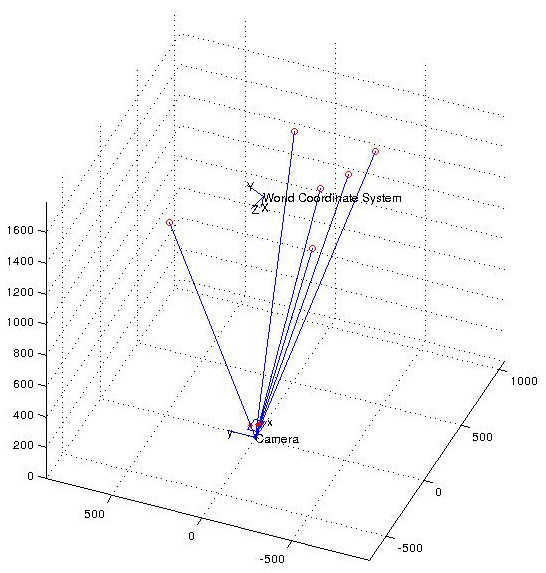
\includegraphics[width=3in]{./pics/part3-1}}
\subfigure{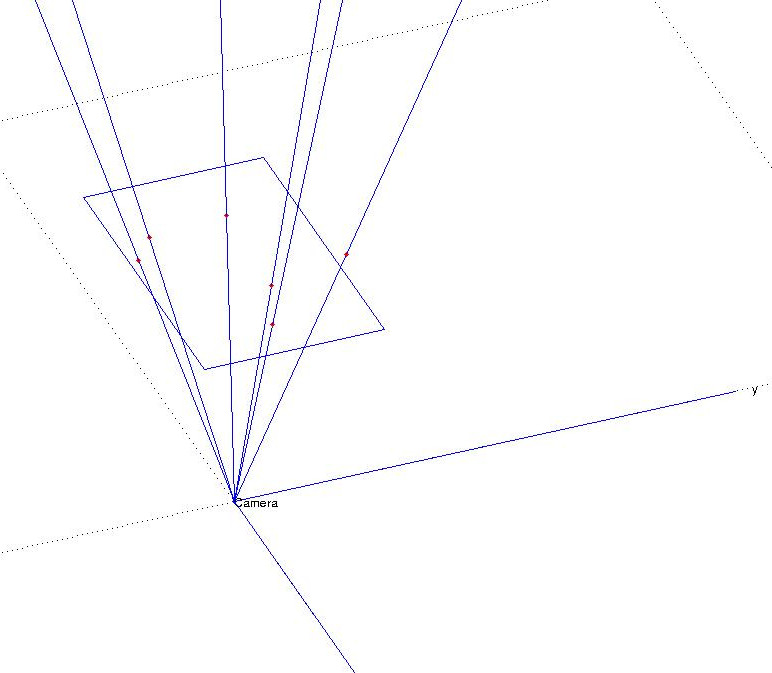
\includegraphics[width=3in]{./pics/part3-2}}
\caption{Obtained results. Left: the whole picture, with correct aspect-ratio. Right: zoomed-in to view the image plane.}
\label{fig:step12}
\end{figure}
We can see that all the optical rays are crossing the 2D points on the image plane. Note that one of the points is outside of the image plane, because the corresponding 3D point is outside of the view. The image on the left is shown keeping the aspect-ratio to demonstrate the coordinate systems and the image on the right is to show the image plane and the projected 2D points.
\section*{Conclusion}
In this laboratory work we studied camera calibration techniques in details. We implemented and tested Hall and Fougeras methods with different number of points and with different additive noise. We illustrated the world with the 3D points, camera and the image plane and understood world to camera and camera to world transformations. Finally we can say that this coursework was very useful to solidify our knowledge in camera calibration and all the steps that we carried out were helpful to better understand the field in more details.
\end{document}
